\section{Phase competition at $p=\alpha=1/2$}
\label{sec:flagship}
\subsection{Front reversal and its resolution}
\label{sec:fronts}

At this representative point the bulk and interfacial evidence are best
resolved. Figure~\ref{fig:flagship} places the complementary observations
on their actual probability scales. In independently prepared strips the
active region retreats at lower $q$ and advances at higher $q$. Near
reversal, its interior retains substantial activity: the fronts bound an
active phase rather than a fragmenting remnant.

The late axial crossing in the independent $10^7$-step cohort is
$q^*=0.04594117$ over $5$--$10\times10^6$ steps. Slopes of integrated bond
activity, interface-site count, and live mass instead locate zeros at
0.04594075, 0.04594075, and 0.04594063. These are different estimators of
the same trajectories; their agreement checks the threshold definition
without adding independent realizations.
The crossing shifts from 0.04593717 in the earlier $2$--$5\times10^6$
window. The threshold-based shift remains positive in a small-sample reference
calculation, whereas the integrated bond-activity shift is smaller and
its interval includes zero (Supplemental Sec.~\ref{S-sec:sfronts}).
The remaining time dependence is therefore estimator-dependent in this
small ensemble; it does not specify an extrapolation law.

For normal directions $(1,0)$, $(2,1)$ and $(1,1)$, crossings lie in the
same narrow probability region. The $L=16384$, $1$--$2\times10^6$ data
give an axial-minus-tilted difference of $4.66\times10^{-6}$ with the
threshold envelope, reduced to $2.70\times10^{-6}$ using integrated bond
activity. The statistical significance depends on the interval method;
the tilted bands also have different physical widths and interface
lengths at fixed $L$. We report these as small finite-geometry contrasts,
not a resolved limiting anisotropy.

We use $q^*=0.04594$ as a rounded operational reference and vary it over
$[0.04592,0.04596]$ for normalization sensitivity. This range encompasses
the available extended-front estimates. It is neither a confidence
interval for a limiting boundary $q_c$ nor a bound on later relaxation.
The detailed orientation and window comparisons are in Supplemental
Sec.~\ref{S-sec:sfronts}.

\begin{figure*}
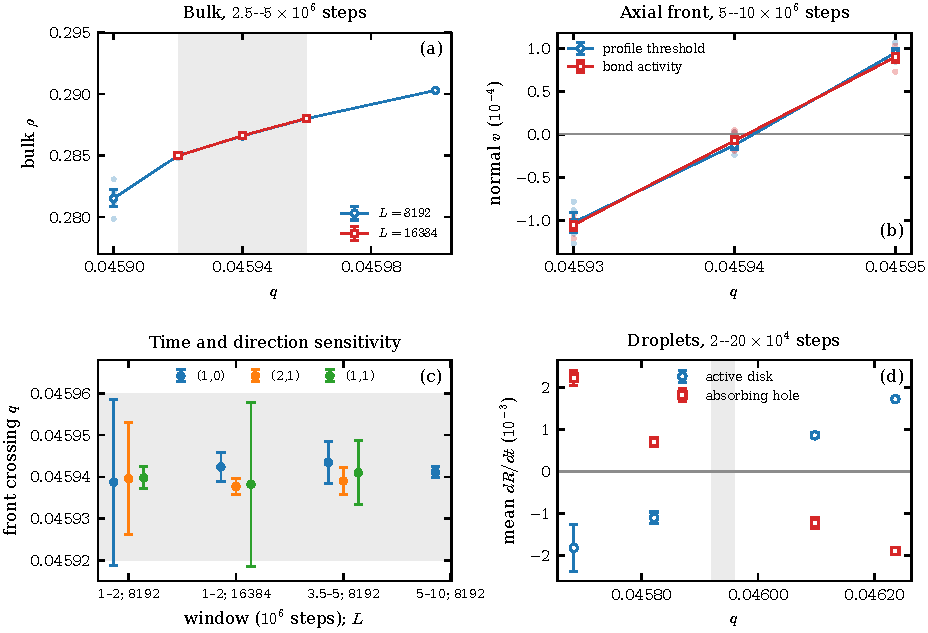
\includegraphics[width=\textwidth]{figs/fig_flagship}
\caption{Bulk and interfacial evidence at $p=\alpha=1/2$, plotted at the actual
probabilities $q$. (a) Unconditional bulk interface density, integrated over
$2.5$--$5\times10^6$ steps separately for each run, at $L=8192$ and 16384.
(b) Axial-front velocities for the independent $L=8192$, $T=10^7$ cohort,
fitted over $5$--$10\times10^6$. The profile-envelope estimate is compared
with the slope of the integrated bond activity, converted to an equivalent
width using the fixed reference density 0.2866. Four independent runs
contribute at every point in (a,b); faint symbols show individual runs and
bars give one standard error. Lines join group means.
(c) Envelope crossing estimates for the stated time windows and sizes.
The $T=2\times10^6$, $5\times10^6$, and $10^7$ cohorts are independent.
Bars are approximate pointwise delta-method Student-$t$ sensitivity intervals
with Welch--Satterthwaite degrees of freedom, conditional on the observed
bracketing pair. Small-sample coverage and bracketing uncertainty remain
limitations. All four runs must retain separated-front geometry throughout
the fit window; no invalid individual run is selectively removed.
(d) Growth rates of an active disk and an absorbing hole of initial radius
1000 on an $L=4096$ lattice, fitted over $2\times10^4$--$2\times10^5$ steps.
Bars are one standard error over four runs. The gray region in (a,c,d) is
the operational reference range $[0.04592,0.04596]$, used for normalization
sensitivity. It is not a confidence interval or an asymptotic bound.
The coarse droplet points in (d) do not resolve the smaller separations
between the front crossings in (c).}
\label{fig:flagship}
\end{figure*}


\subsection{A persistent dynamically active bulk}
\label{sec:bulk}

At $q=0.04594$, all four random-start $L=8192$ runs remain active through
$5\times10^6$ steps, with time-weighted mean $\rho=0.28659$ over the
last half. At $L=16384$, the corresponding four-run mean is 0.28661.
The means at the nearby $q=0.04592$ and 0.04596 are 0.28498 and 0.28803;
none of these twelve largest-system runs absorbs. Their late-window
density changes show no consistent decrease across the cohorts.
At the central probability, the actual fraction of sites flipping per
step has late mean 0.20874. The measured branch therefore retains
microscopic activity, independently of the bound in
Eq.~\eqref{eq:activitybound}.

The final configurations supply a spatial check.
At $q=0.04594$, $C(128)\simeq0.0046$ at both $L=8192$ and 16384;
the largest-system correlation drops from 0.427 at one spacing to
$5.7\times10^{-4}$ at $r=256$, with signed fluctuations about zero at
longer separations. The magnetic second-moment ratios on doubling size
are near one in a common late window (Supplemental Sec.~\ref{S-sec:sbulk}).
These are finite-scale checks at the sampled probabilities, not a
correlation-length extrapolation or an exclusion of every possible
intermediate critical regime.

On the lower-$q$ side the bulk exhibits delayed collapse accompanied by
the growth of absorbing domains [Fig.~\ref{fig:snap}(b)]. At
$q=0.045441$, for example, the mean time of recorded half-density loss
approaches $6.7\times10^4$ steps at the largest sampled sizes,
consistent with many droplets nucleating and growing locally.
Absorbing domains of opposite type leave active walls between them, so
half-density loss occurs before consensus.
On the active side, finite-volume survival instead increases strongly
with size. In independent $10^7$-step cohorts at $q=0.046359$, consensus
counts are $(32,32,6,0)$ out of 32 at $L=(64,128,192,256)$; at
$q=0.04605$ they are $(15,6,0)$ out of 16 at $L=(192,256,384)$ through
$3\times10^6$ steps. These size contrasts support a stable active branch
on the observed scales, but do not determine an asymptotic lifetime law.

\subsection{Opposing invasion and finite droplets}
\label{sec:opposing}

A disordered disk of radius $1000$ in the dead phase and a dead hole of
the same radius in an active background exchange growth directions
across the reversal region. All 32 trajectories, four for each geometry
at four probabilities, have the reported sign. The nearest sampled probabilities on opposite sides of reversal are 0.0458221 and 0.0460979; their separation,
$2.758\times10^{-4}$, is much wider than the directional crossing
differences. These measurements establish opposite invasion on the
sampled flanks. Radius traces and the curvature-law comparison are in
Supplemental Fig.~\ref{S-fig:drop2}.

They do not resolve an orientation-dependent coexistence interval.
Even for one isotropic zero, the model
$\ds R/\ds t=\pm v-D/R$ predicts shrinkage of both finite droplets
when $|v|<D/R$. With $D\simeq0.20$, $R=1000$ and the local axial
slope $\ds v/\ds q\simeq10.75$, this curvature-only full width is
about $3.7\times10^{-5}$ in $q$. Inferring generic coexistence from
droplet shrinkage would require sampling the candidate interval and
increasing the radius~\cite{wang2015,liu2018}.
Together, the finite bulk density, coherent invasion, and delayed
nucleation-driven decay provide the numerical case for a discontinuous
transition here. The precision of a unique limiting boundary is a
separate question.
